\documentclass[a4paper,10pt]{article}

%\VignetteIndexEntry{PREDA S4-classes}

\usepackage[latin1]{inputenc}
\usepackage[english]{babel}
\usepackage{fontenc}
\usepackage{graphicx}

\title{PREDA S4-classes}
\author{Francesco Ferrari}

\usepackage{Sweave}
\begin{document}
\maketitle

\begin{abstract}
This document provides a description of custom S4 classes used to manage data structures for PREDA: an R package for Position RElated Data Analysis.
The PREDA package is used for the integrative analysis of functional genomics data and their genomic positions, in order to identify position-related trends in data: i.e. to identify differentially expressed genomic regions in specific cell contexts or as a consequence of chromosomal aberrations in cancer. To perform this position-related analysis of genomics data, custom data structures to manage genomic data and genomic annotations (i.e. positions) are required. Custom S4 classes have been implemented to achieve a flexible and powerful informatic infrastructures, with user frendly functions developed to facilitate the analyses.
\end{abstract}


\tableofcontents

\newpage


\section{PREDA S4-classes overview}

The PREDA package is used for Position RElated Data Analysis in functional genomics studies. For example PREDA can be used to identify differentially expressed genomic regions, as a consequence of chromosomal aberrations in cancer cells. Or to identify genomic regions with specific characteristics, such as altered copy number values.

The algorithm implemented in the PREDA package consists of three main steps:
\begin{enumerate}
\item 
adoption of a statistic for each gene (or other genomic feature under investigation);
\item 
smoothing of the statistic along the chromosomal position of the corresponding genes using non linear regression methods;
\item
application of permutations to identify chromosomal regions with significant positive or negative peaks of the selected smoothed statistic, with corrections for multiple tests.
\end{enumerate}


Custom S4-classes were defined to manage input and output data of PREDA analyses. Each of the custom S4-classes used for input and output data are actually defined as extensions of each other: so as to maximize the methods inheritance between objects of different classes (fig. \ref{fig:PREDA_inputClasses}, fig. \ref{fig:PREDA_outputClasses} and fig. \ref{fig:PREDA_inputoutputClasses}).



\section{Data structures for input data}

The basic input for position related analysis of genomic data is constituted by data structures that can manage genomic data and structures to manage genomic annotations, i.e. the association between each point of data and its mapping on the genome.
In particular statistics computed on genomics data are used as input data: such as statistics accounting for differential expression, if the analysis aims at identifying differentially expressed genomic regions. These statistics computed on the genomic data under investigation are managed with the S4-class \texttt{StatisticsForPREDA}. Then, the genomic annotations required for the analyses are basically the positions associated to each data point that are managed in the PREDA package using S4-classes \texttt{GenomicAnnotations} and \texttt{GenomicAnnotationsForPREDA} (see the following sections for details).
Finally the S4-class \texttt{DataForPREDA} results from merging data and annotations from the other classes.

\subsection{Genomic annotations}

The essential genomic annotation required to analyze the relationship between genomic data and positions is the actual chromosomal position associated to each genomic feature under investigation. For example if the analyzed data are gene expression profiles, then the essential genomic annotations are the genomic coordinates of each gene, in term of chromosome, strand, start and end position of each gene locus.

\subsubsection{GenomicAnnotations-class}

The main slots of \texttt{GenomicAnnotations} S4-class objects are the slots containing genomic coordinates: \texttt{chromosome}, \texttt{strand}, \texttt{start} and \texttt{end} slots, holding the position of each genomic feature. Each element must be identified by a unique id contained in the \texttt{ids} slot. This ids will be used to match annotations and genomic data. For example in the analysis of gene expression data, the ids will usually be the probe identifiers, whereas genomic coordinates will be the genomic positions of each gene locus. See also the class manual page within the PREDA package for further details about each slot.


\subsubsection{GenomicAnnotationsForPREDA-class}

The \texttt{GenomicAnnotations} S4-class provides an R representation of genomics annotations with a biological meaning: the start and end positions identify he chromosomal localization of each gene locus (or other genomic feature) under investigation. Moreover these annotation are familiar concepts commonly handled by molecular biologists to describe genomic data annotations.
However, smoothing analysis, that is the core of PREDA analysis procedure, requires a unique position associated to each data point. For this reason, genomic annotations must be enriched by specifying which exact position should be associated to each gene when performing the smoothing analysis. For this purpose, the \texttt{GenomicAnnotationsForPREDA} S4-class extends the \texttt{GenomicAnnotations} class with just one additional slot: the \texttt{position} slot, holding the reference position that will be used for smoothing (fig. \ref{fig:PREDA_inputClasses}). Tipical choices for the reference position include i) the median position between start and end coordinates of each gene; ii) the start coordinate of each gene; iii) the end coordinate of each gene; iv) alternative choice of the start coordinate if the gene is on positive strand or of the end coordinate if the gene is on the reverse strand. The user can chose the reference positions according with the data under investigation and analysis purpose. Specific functions in the PREDA package facilitate the user in generating reference positions from genomic annotations.


\subsection{Genomic data}
Genomics data coming from high throughput technologies (microarray or sequencing based technologies) are usually associated to their genomic annotations using a set of unique identifiers (ids). This is the same approach adopted in PREDA: objects holding genomics annotations contain an \texttt{ids} slot and objects containing genomic data have an \texttt{ids} slot as well that is used to match data and annotations.


\subsubsection{StatisticsForPREDA-class}
Usually genomics data (such as gene expression data) are not used as is, whereas different statistics are computed on data in order to address distinct problems. For example, if the analysis is focused on differential gene expression, then proper statistical scores are computed to identify differentially expressed genes. Similarly, for PREDA analysis, different statistical scores can be computed on raw genomic data, depending on the purpose of the study, and used as input statistics for position related analysis. The statistical score computed on each gene (or other genomic feature) under investigation is stored and managed with \texttt{StatisticsForPREDA} objects. These objects basically includes the genomic data (\texttt{statistic} slot) and the ids associated to each element (fig. \ref{fig:PREDA_inputClasses}). For example, if the analysis aims at identifying differentially expressed genomic regions, the t statistic can be computed for each gene and included in a \texttt{StatisticsForPREDA} object. This class can also store and manage multiple statistics, e.g. associated to multiple samples under investigation, because the \texttt{statistic} slot contains actually a matrix object. See also the class manual page within the PREDA package for further details about each slot.


\subsection{Genomic data and annotations}
A custom class to manage all of the input data required for PREDA analysis, i.e. genomic annotations and genomic data, has been defined as well to achieve a more user friendly procedure.

\subsubsection{DataForPREDA-class}
The \texttt{DataForPREDA} S4-class is actually defined as an exact extension of the classes \texttt{GenomicAnnotationsForPREDA} and \texttt{StatisticsForPREDA}: therefore this class includes all of the slots from the parent classes without any additional slot (fig. \ref{fig:PREDA_inputClasses}). The PREDA pacakge includes user friendly functions allowing to easily merge genomic annotations and data into a \texttt{DataForPREDA} object, implementing as well the filtering of unmatched elements (ids).



\begin{figure}[htbp]
 \centering
 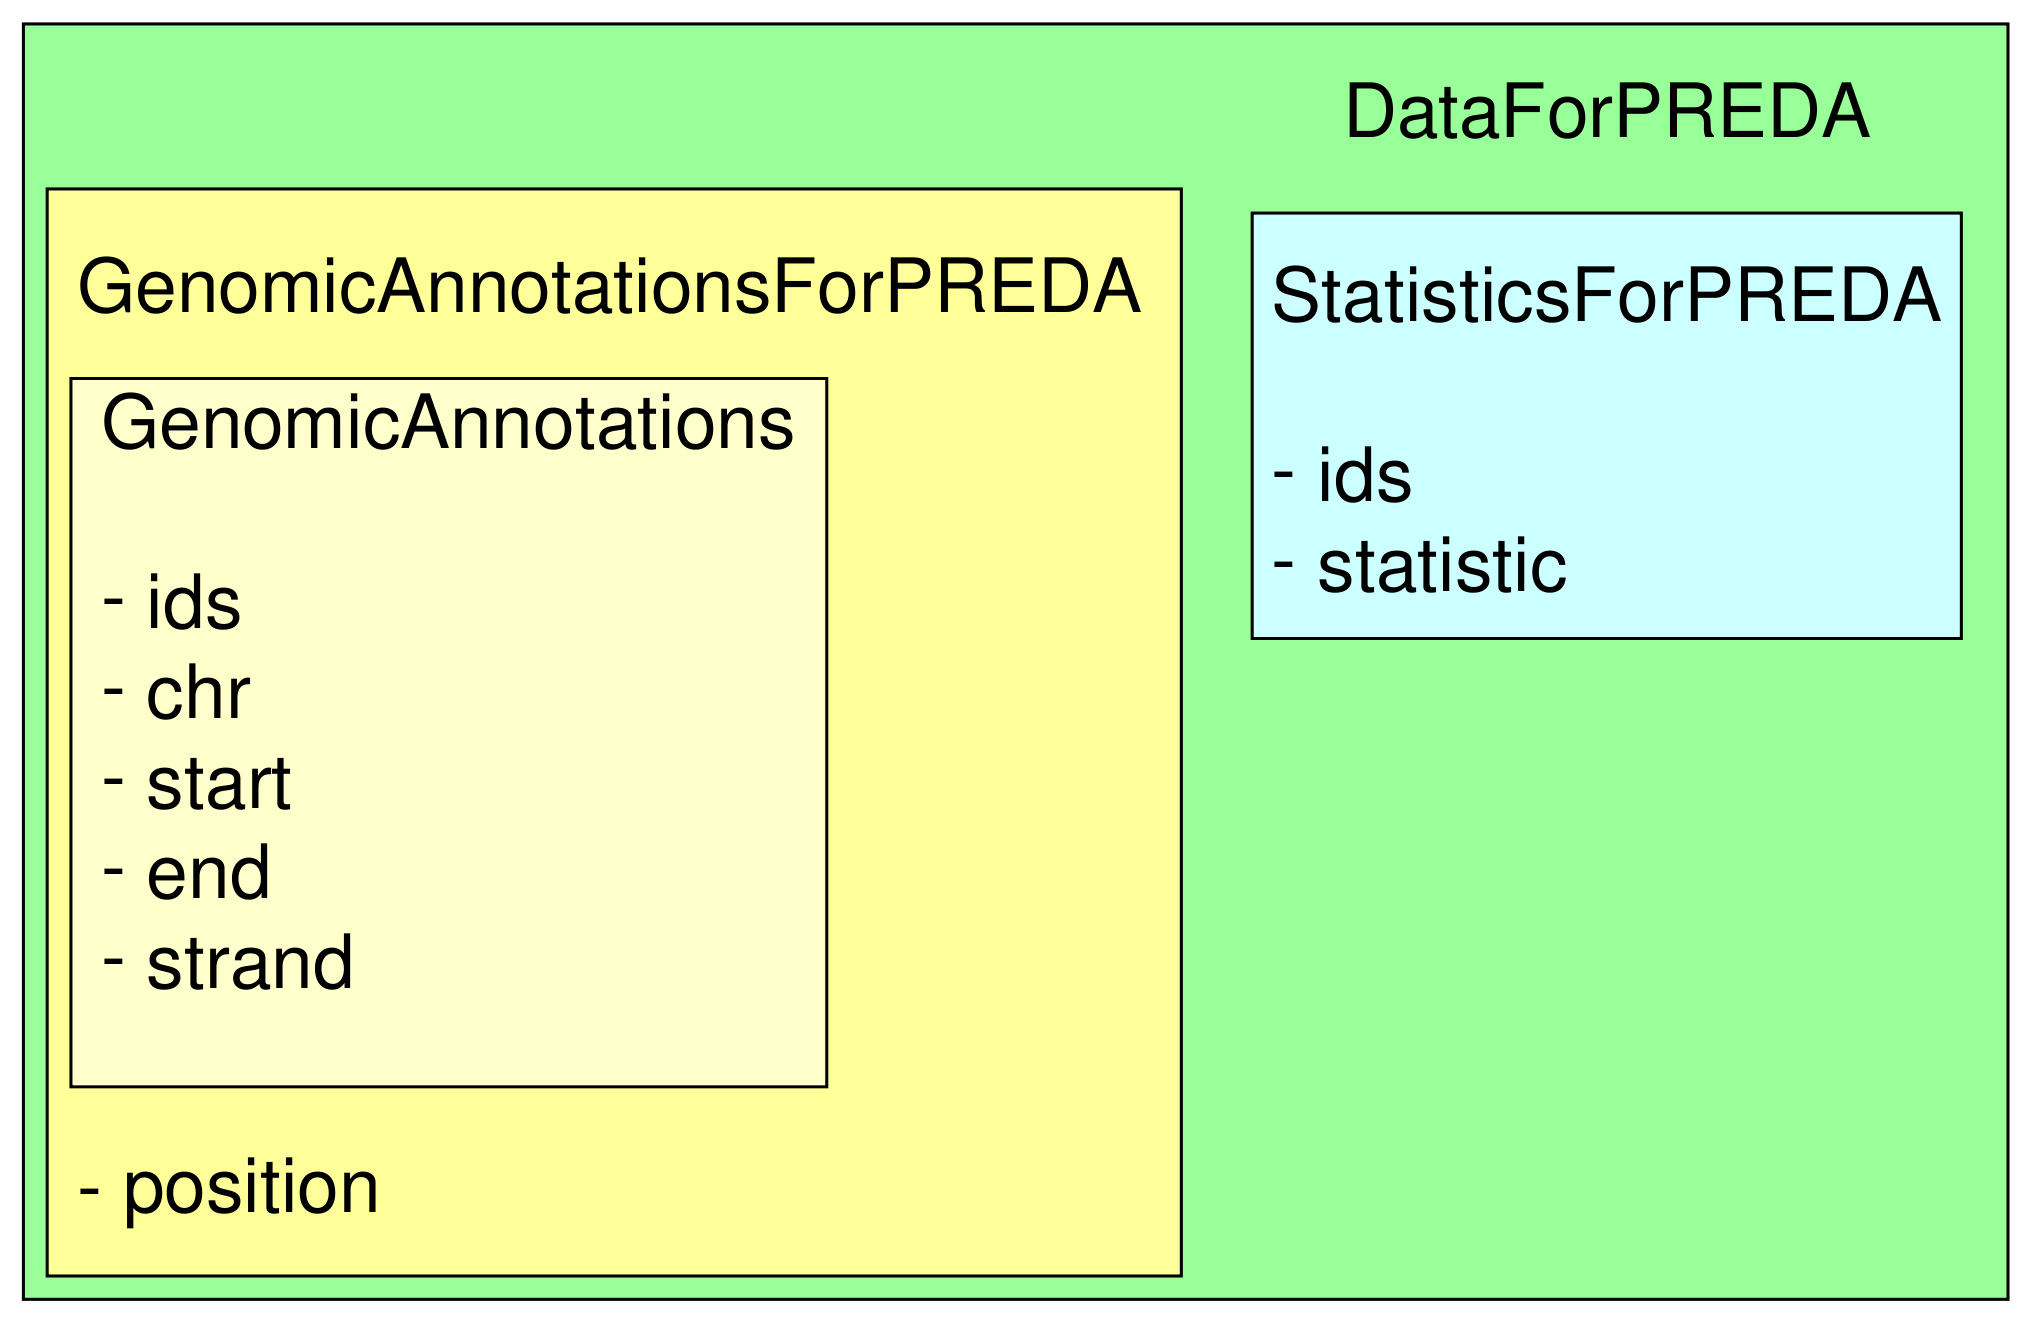
\includegraphics[width=9cm]{images/PREDA_inputClasses.png}
  \caption{PREDA: S4-classes for input data. Classes are designed as extensions of each other to maximize methods inheritance. Classes extending other classes are represented as concentric squares.}
 \label{fig:PREDA_inputClasses}
\end{figure}


\section{Data structures for output data}
The fundamental output of the analysis is basically a set of genomic regions with significant modifications in the genomics data under investigation (used as input statistics). This results can be managed as an object of class \texttt{GenomicRegions}. Moreover, other S4-classes named \texttt{PREDAResults} and \texttt{PREDADataAndResults} are available to manage the complete set of statistics and scores that are computed during PREDA analysis.


\subsection{PREDA results}
The \texttt{DataForPREDA} objects, conveniently store all of the input data for PREDA analysis. Similarly \texttt{PREDADataAndResults} or \texttt{PREDAResults} can store all of the output data from PREDA: i.e. the output of \texttt{PREDA\_main()} function, that performs the core of the analysis.


\subsubsection{PREDADataAndResults-class}
The \texttt{PREDADataAndResults} S4-class is an extension of \texttt{DataForPREDA}: therefore it includes all of the slots holding input data (both genomic data and annotations), along with the complete set of statistics computed during PREDA analysis (fig. \ref{fig:PREDA_inputoutputClasses}). The basic output of PREDA is constituted by the smoothing results of input statistic, the p-values and the adjusted p-values (q-values) associated for each genomic position. These output statistics are stored in the slots \texttt{smoothStatistic}, \texttt{pvalue} and \texttt{qvalue}, respectively. This objects can actually hold results concerning multiple samples (multiple RPEDA analyses) because these slots contain actually matrix objects, similarly to the \texttt{statistic} slot in input data objects. See also the class manual page within the PREDA package for further details about each slot.


\begin{figure}[htbp]
 \centering
 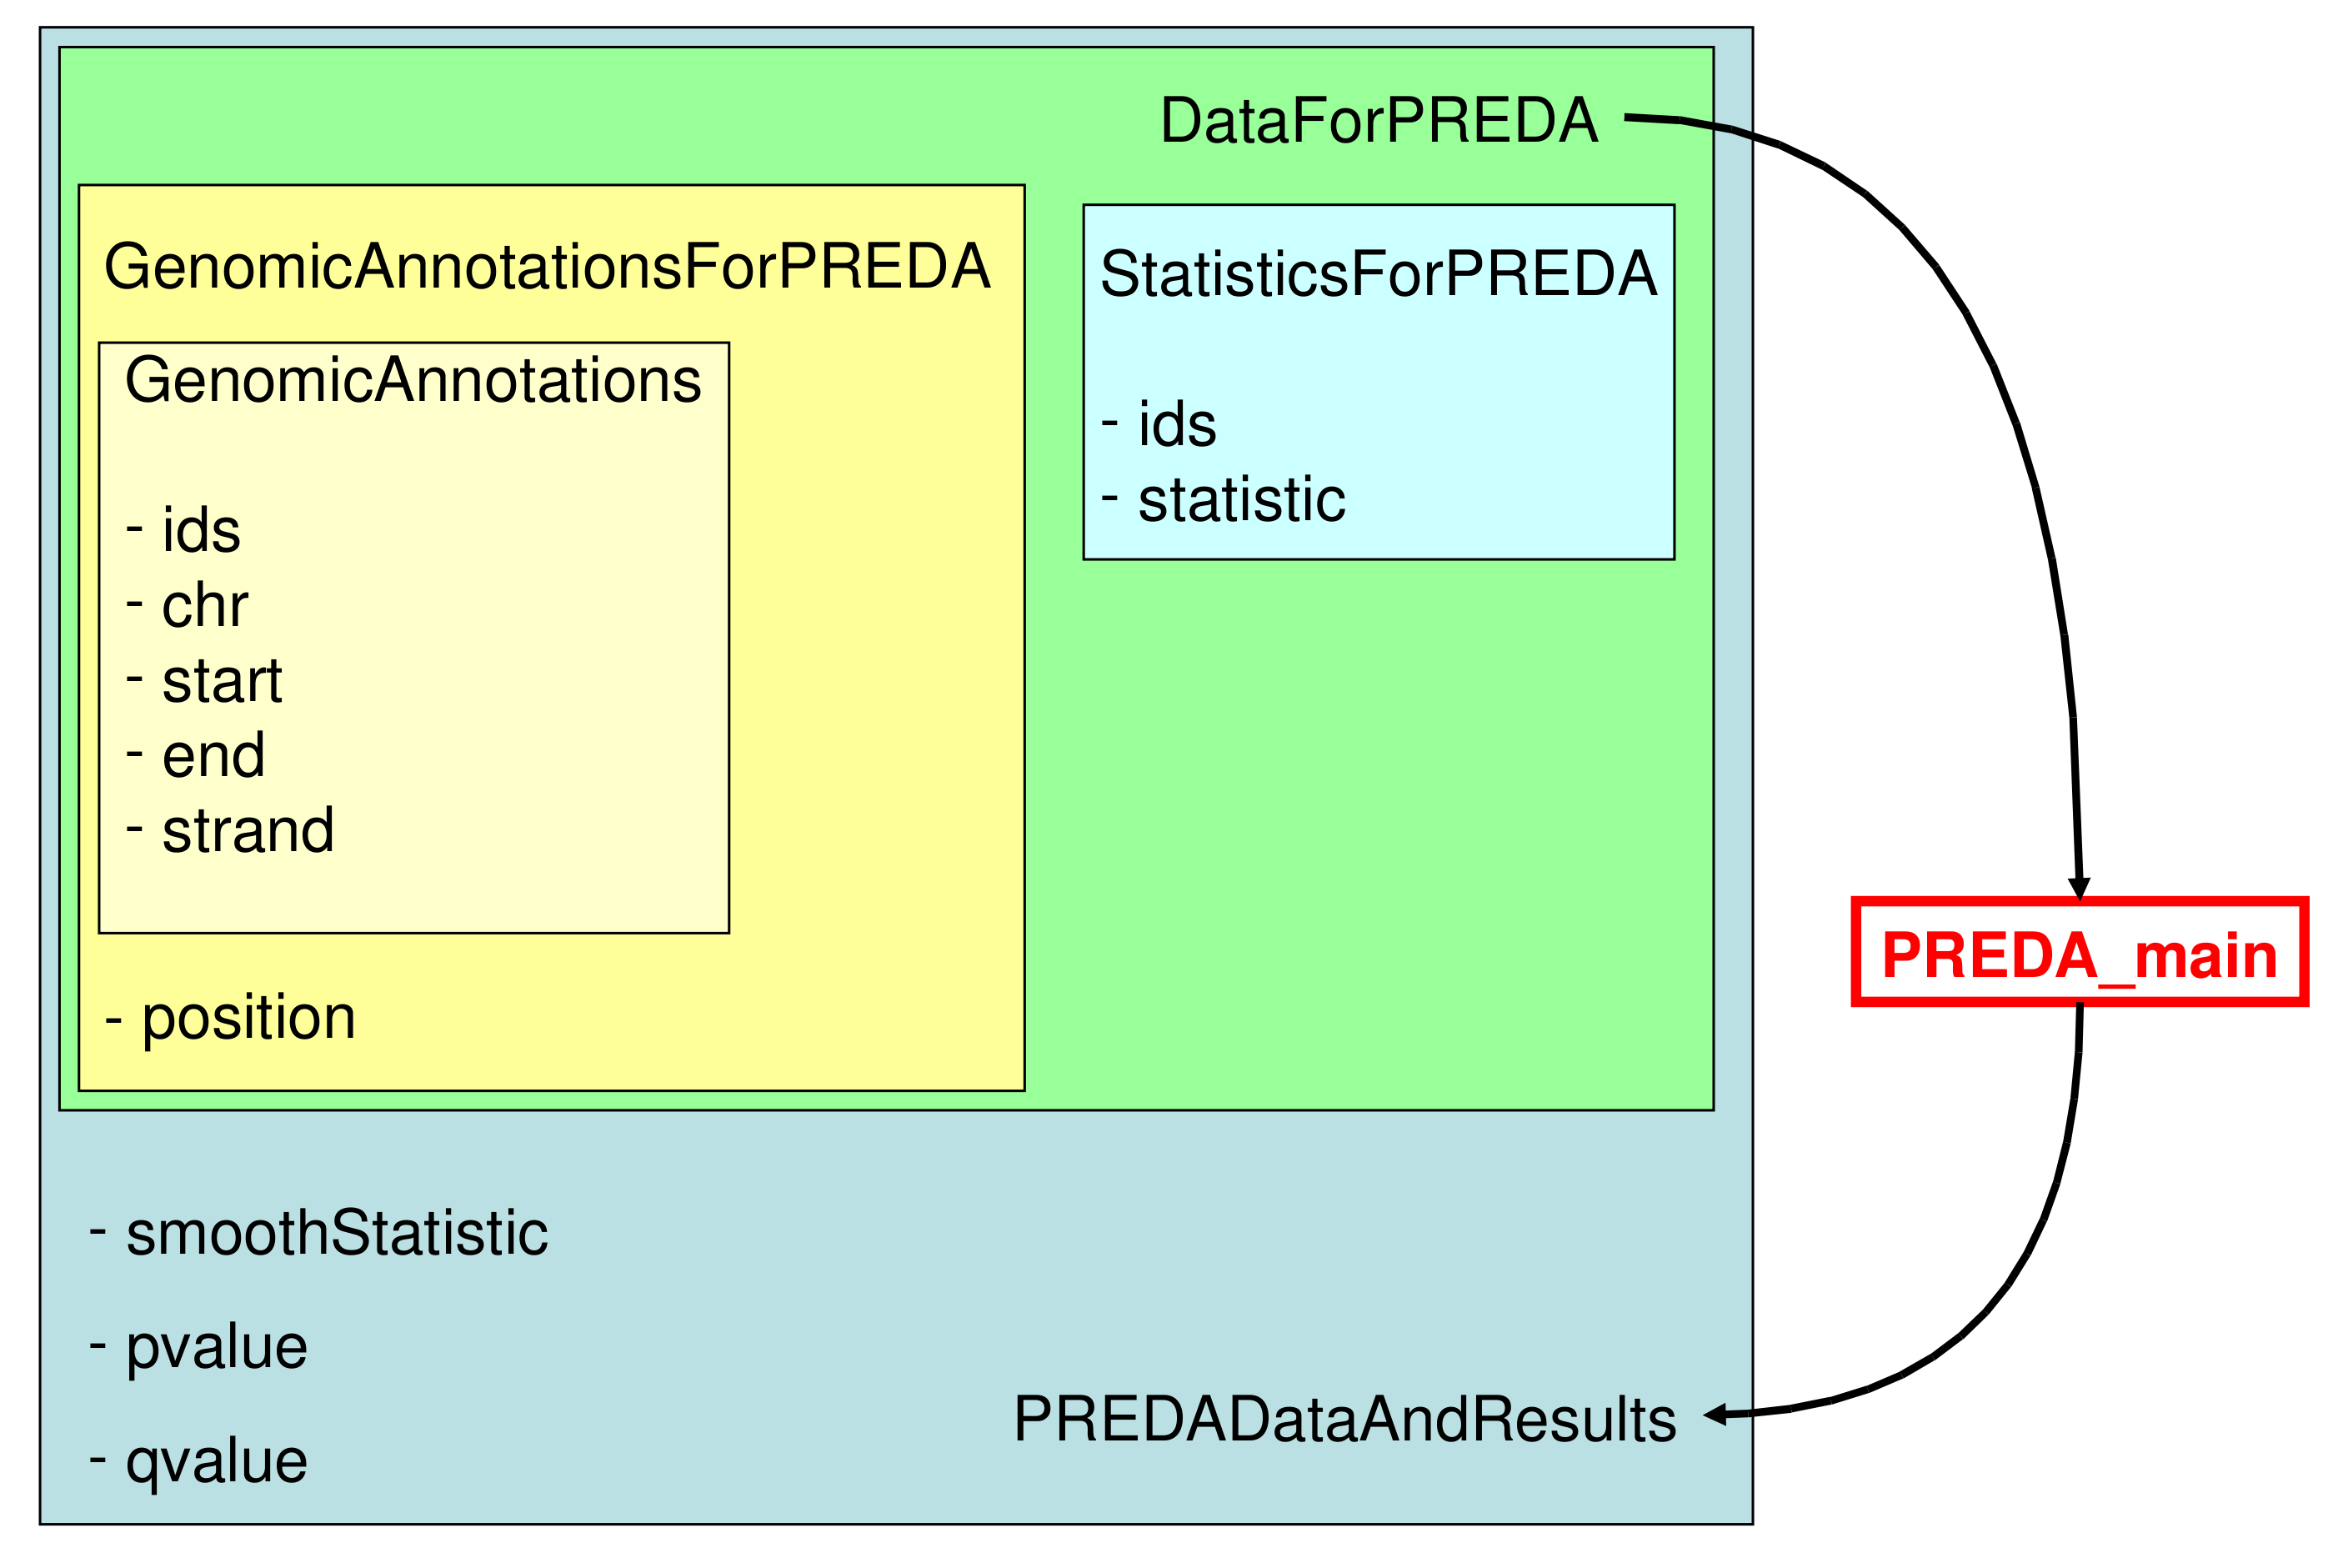
\includegraphics[width=9cm]{images/PREDA_inputoutputClasses.png}
  \caption{PREDA: S4-classes for input and output data. Classes are designed as extensions of each other to maximize methods inheritance. Classes extending other classes are represented as concentric squares.}
 \label{fig:PREDA_inputoutputClasses}
\end{figure}


\subsubsection{PREDAResults-class}

For some applications, the input statistic is not included in the output data because the PREDA statistics (\texttt{smoothStatistic}, \texttt{pvalue} and \texttt{qvalue}) are estimated at a set of genomic positions that is different from the input set of genomic coordinates (see also the SODEGIR procedure in the PREDA tutorial for an example) (fig. \ref{fig:PREDA_outputClasses}).

\begin{figure}[htbp]
 \centering
 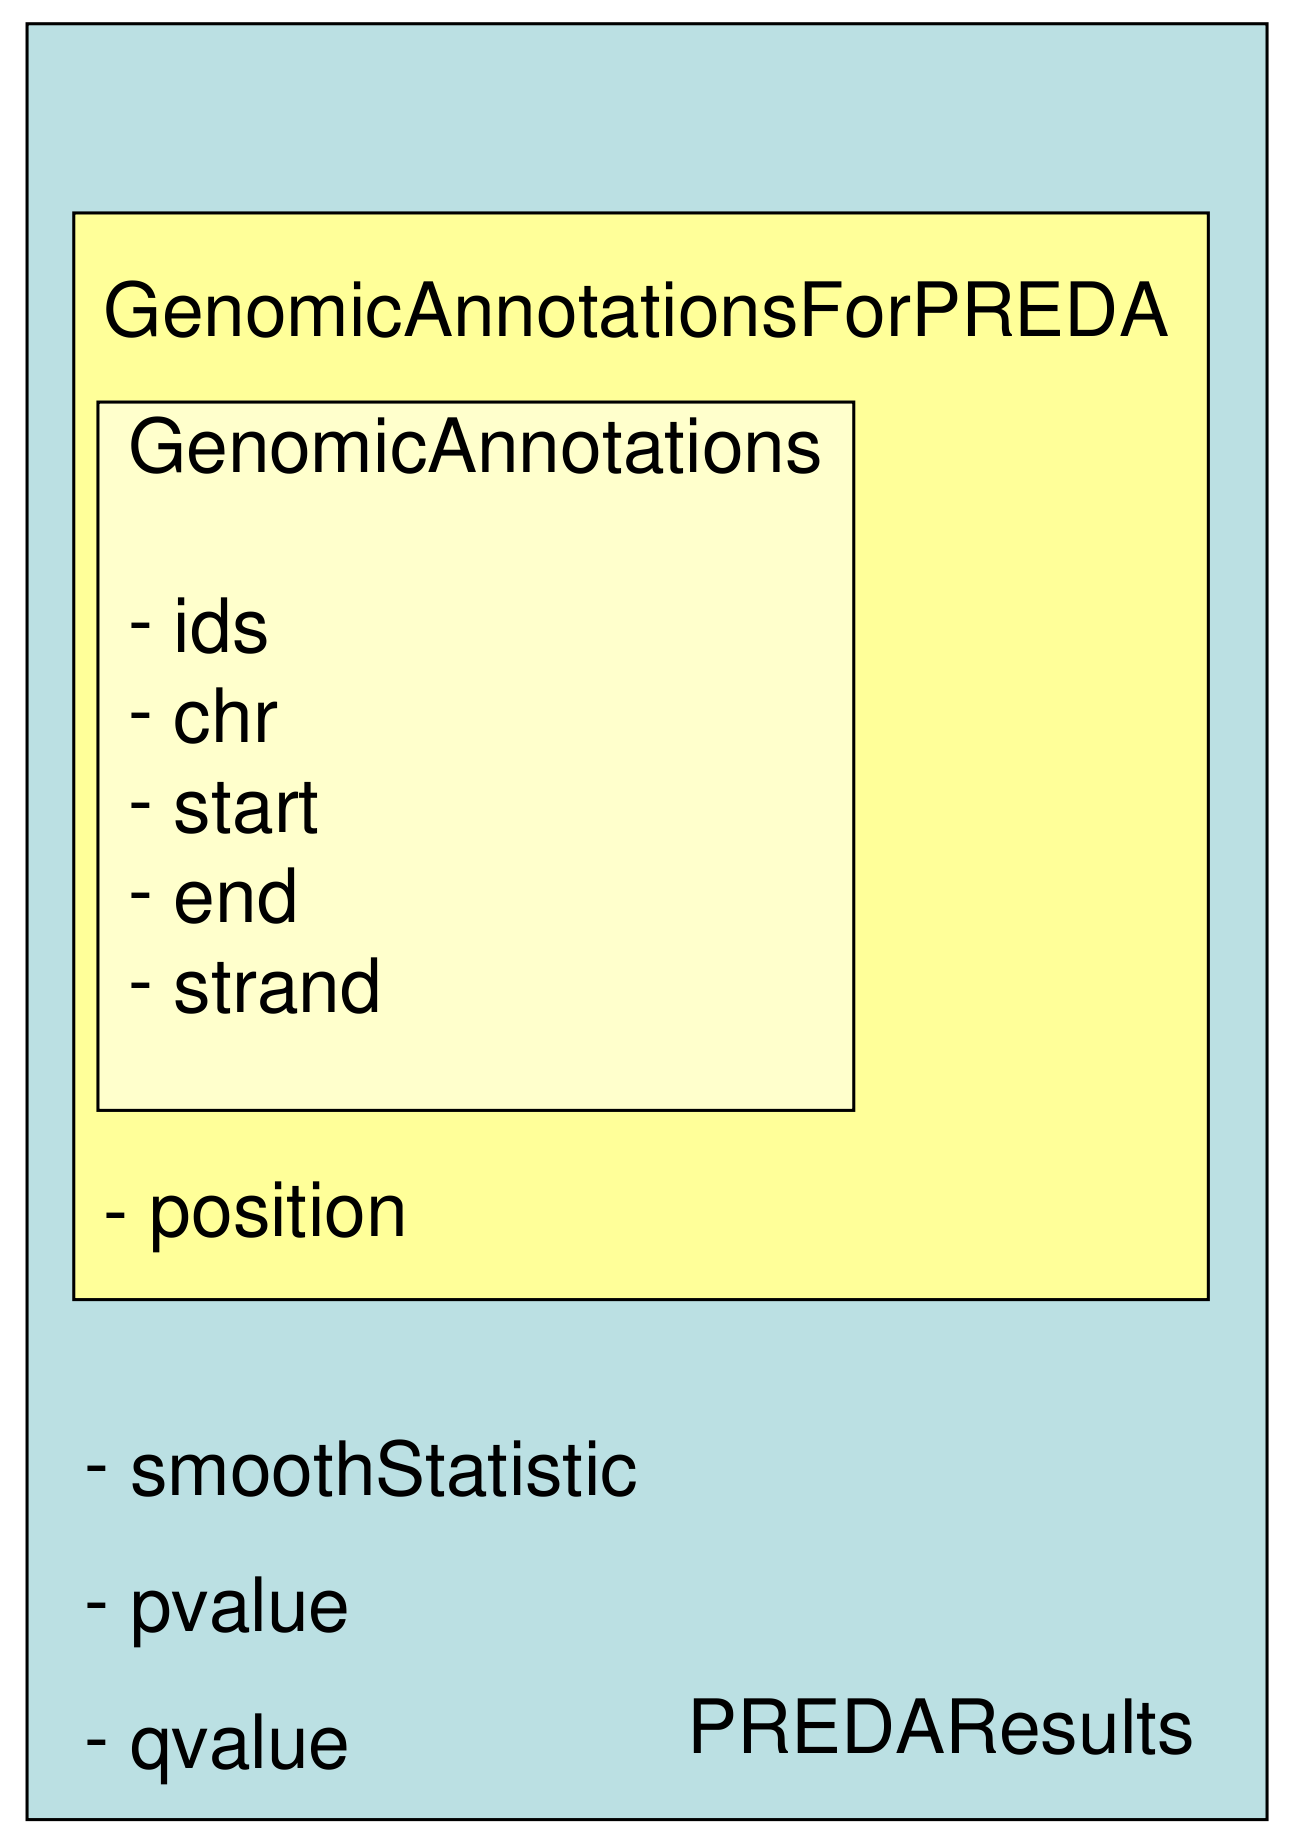
\includegraphics[width=5cm]{images/PREDA_outputClasses.png}
  \caption{PREDA: S4-classes for output data. Classes are designed as extensions of each other to maximize methods inheritance. Classes extending other classes are represented as concentric squares.}
 \label{fig:PREDA_outputClasses}
\end{figure}


\subsection{Genomic regions}
The \texttt{PREDADataAndResults} and \texttt{PREDAResults} objects contain the relevant output of PREDA analysis in a data structure that is easily managed within the package informatic infrasctructure. Nevertheless, the real biological meaningful output of the analysis is expected to be a set of genomic regions with significan variations in the analyzed statistic on genomic data. This biological meaningful entity is well represented by the \texttt{GenomicRegions} objects.

\subsubsection{GenomicRegions-class}

The essential content of \texttt{GenomicRegions} objects are the slots holding chromosome, start and end positions of a specific set of genomic regions. This is the basic data structure used to deliver results and can be used as well to draw genomic plots or to compare results from different analyses (including third party analysis reported in literature articles). Other optional slots for this class can be used to hold additional annotations about the set of genomic regions.  See also the class manual page within the PREDA package for further details about each slot.

% \addcontentsline{toc}{section}{References}
% \bibliographystyle{unsrt}
% \bibliography{PREDA}


\end{document}


